In the model proposed below, the weight of the disk galaxy is supported by the turbulence injected by supernoave.
This links density and star formation together; a higher gas density leads to leads to more star formation and hence a higher supernovae rate.
This higher supernova rate injects more turbulence into the system (i.e. a higher pressure), expanding the gas and decreasing the pressure.
Under an equilibrium situation, there can be a relation formed between the surface star formation rate and surface gas density.

Once this star formation relation (which is similar to the Kennicutt-Schmidt law described above) has been formulated, it can be combined with calibration simulations provided by \citet{martizzi_supernova_2015} that give the relation between dispersion injected from supernovae and surface gas density to produce an effective equation of state, which is found to have a polytropic index of $\gamma_eff = 5/4$.

\begin{figure}[!ht]
    \centering
    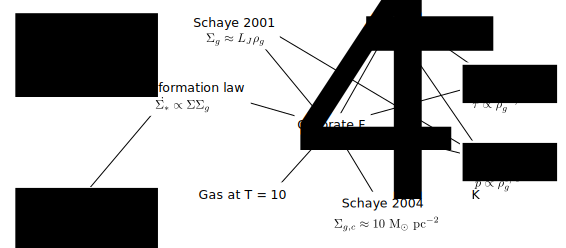
\includegraphics[width=\textwidth]{flowchart.pdf}
    \caption{This flowchart shows the links between the various components of the model and their respective references.
    It may be useful to the reader as they progress through the rest of this chapter, as a number of elements are required at any one time.}
    \label{fig:flowchart}
\end{figure}
